











Introduction
Content: Introduce the importance of anonymous credentials for privacy-preserving authentication. Highlight challenges: efficiency of expressive proofs, multi-issuer support, Sybil resistance, and trust distribution.
Narrative Role: Sets the stage, motivating why your contributions matter.
Suggestion: Expand to include a roadmap of your contributions and their progression.



Story Overview
\begin{enumerate}
    \item Chapter 2: Foundations: Optimized Expressive Predicate Proofs \\
    We need efficient, expressive proofs for credentials, so I optimized PS signatures
    
\end{enumerate}

























\section*{Thesis Roadmap}

This thesis explores anonymous credential systems, emphasizing efficiency, security, and real-world utility. We start with an efficiency analysis of predicate proofs in anonymous credentials using AGM security and benchmarks (Section 1). Next, we introduce MIMC-ABC, a multi-issuer system for privacy-preserving identity binding (Section 2). We then extend it with a hierarchical structure for managing complex credentials securely (Section 3). To address sybil attacks and revocation, we propose the Credential Relationship Bound Nullifier (Section 4). Finally, tMIMC-ABC decentralizes issuance with a threshold approach, enhancing security and efficiency (Section 5).

% \section*{Thesis Roadmap}

This thesis advances anonymous credential systems through a series of connected contributions focusing on efficiency, security, and practical deployment:

\begin{itemize}
    \item \textbf{Chapter 1: Efficient Predicate Proofs in Attribute-Based Anonymous Credentials (ABC)}
    
    Gap Analysis: Most Expressive and Efficient, Secure ABC. 
    
    % We're choosing this because it's expressive, efficient, and secure, we also optimized it to make it even better.
    
    \begin{itemize}
        \item compare the expressiveness of ABC's - reasoning why sigma protocols for committed exponents are most expressive. 
        
        \item compare the efficiency of BBS+, PS variants, show ours is the most efficient variant for show/verify
    
        \item Security analysis of our position binding commitments and rerandomizable signature in the Algebraic Group Model
        
        \item First comprehensive benchmarks comparing the variants of BBS+ and PS signature schemes for predicate proofs

        \item we have the most efficient PS variant for show/verify
        
        \item practical improvements: analysed schnorr proofs and show it's actually logarithmic practically. Analyzed Pairing with optimization and showed it's linear but not as bad.
        
    \end{itemize}

    \item \textbf{Chapter 2: MIMC-ABC for Multi-Issuer Identity Binding}
    \begin{itemize}
        \item is proven secure, extended by security of base
        \item Security analysis proving resilience against forgery and identity
    \end{itemize}

    \item \textbf{Chapter 3: Hierarchical MIMC-ABC for Identity System}
    \begin{itemize}
        \item Formal definition of credential hierarchy supporting master and sub-credentials
        \item Secure private key issuance protocol preserving unlinkability while maintaining hierarchy
    \end{itemize}

    \item \textbf{Chapter 4: Sybil Resistance and Revocation in MIMC-ABC}
    \begin{itemize}
        \item Credential Relationship Bound Nullifier (CRBN) preventing duplicate credential useÍ
        \item Privacy-preserving revocation mechanism with minimal verifier overhead
        \item Security analysis of sybil resistance properties
    \end{itemize}

    \item \textbf{Chapter 5: tMIMC-ABC: Threshold MIMC-ABC}
    \begin{itemize}
        \item Efficient threshold issuance construction outperforming comparable systems
        \item Decentralized identity binding maintaining privacy and integrity
    \end{itemize}
\end{itemize}

Each chapter builds upon previous work, creating a comprehensive framework for secure, efficient, and practical anonymous credential systems suitable for modern distributed environments.

\section{Intro}
\subsection{Problem}
Our research addresses the secure and private verification of complex identity assertions using multiple digital credentials from different issuers. The system ensures all credentials are bound to the same identity and, additionally, supports credential relationship binding to prove structured relationships between credentials while preserving privacy through anonymous authentication.

% We introduce the Multi-Issuer Multi-Credential Attribute-Based Anonymous Credential (MIMC-ABC) system, a novel framework for privacy-preserving identity verification. Unlike single-issuer systems like Idemix, MIMC-ABC enables users to combine credentials from multiple issuers without coordination, using rerandomizable Pointcheval-Sanders signatures and commitments. Our system supports expressive predicates (e.g., "age > 18 AND degree = 'BS'") via zero-knowledge proofs. We prove unforgeability and anonymity—even against malicious issuers—in the Algebraic Group Model, addressing key limitations in prior work and aligning with emerging digital identity needs.

\subsubsection{Problem}

Non-digital identity interactions 

The privacy of non-digital identity interactions is often overlooked. Although users may need to present multiple physical identity documents to satisfy a verification requirement, oftentimes, our identity documents will be verified in plain sight and not digitally recorded. During the interaction, the verifier will check identity binding (that both identity documents are for the same person) and that the user provided different types of identity documents. This interaction is anonymous in many ways and unlinkable. 

Traditional identity systems fail to preserve the privacy of the user but retain accountability of the user 
Traditional systems fail to balance privacy, security, and accountability in these multi-issuer scenarios.

\subsubsection{Key dimensions of the problem}
\begin{itemize}
    \item \textbf{Multi-Issuer Multi-Credentials} The need for MIMC stems from the need to combine credentials issued by various issuers such as a government, university, or private issuers and combine multiple credentials together such as having a valid driver's license and healthcare card to satisfy a government requirement. 

    \item \textbf{Identity binding} Ensuring all credentials in a presentation belong to the same identity without compromising privacy or requiring issuer coordination. Without Identity Binding, an attacker could mix credentials from different individuals to falsely satisfy a verification requirement. Especially important in a multi-issuer setting where different users may have equivalent attributes 

    \item \textbf{Credential Relationship Binding}: Beyond linking credentials to a single identity, users often need to prove structured relationships between credentials (e.g., one credential derived from another or a dependency between them). This property supports advanced use cases, such as nullifiers for Sybil-resistant systems or hierarchical credential verification.

    \item \textbf{Anonymity} Users need to present credentials anonymously, ensuring that different presentations (e.g., to different service providers) cannot be linked to the same individual unless intended and that the underlying credential values not used openly. This protects against tracking and profiling, a growing concern in digital systems. preventing different presentations from being linked to the same individual while maintaining essential security properties


\end{itemize}

\subsection{Related Work}
Compare with TACT, Coconut, Idemix, how we improve on them

\subsection{Motivation}

Traditional centralized identity systems expose users to privacy risks (e.g., data breaches) and lack flexibility for multi-issuer scenarios. Existing anonymous credential systems, while privacy-focused, often assume a single issuer or fail to efficiently integrate multiple credentials with features like Sybil resistance and revocation. As digital identity frameworks, such as the EU’s Mandatory Digital Identity Wallet, push for privacy-preserving solutions, there is an urgent need for a system that supports the complexity of real-world identity use cases—where users juggle multiple online credentials—while ensuring security, privacy, and accountability


Related Work
\begin{figure}
    \centering
    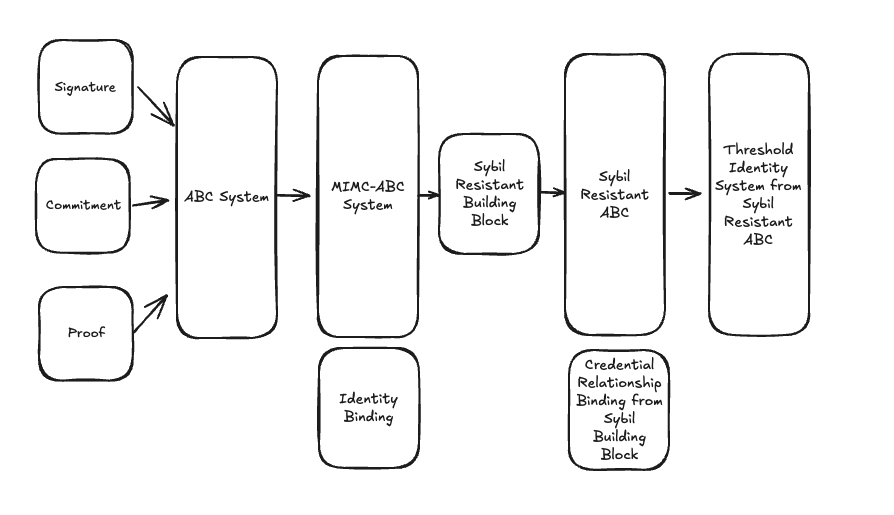
\includegraphics[width=0.75\linewidth]{contribution-illustration.png}
    \caption{Contribution Illustration}
    \label{fig:constribution-illustration}
\end{figure}